% Options for packages loaded elsewhere
\PassOptionsToPackage{unicode}{hyperref}
\PassOptionsToPackage{hyphens}{url}
%
\documentclass[
]{article}
\usepackage{amsmath,amssymb}
\usepackage{lmodern}
\usepackage{iftex}
\ifPDFTeX
  \usepackage[T1]{fontenc}
  \usepackage[utf8]{inputenc}
  \usepackage{textcomp} % provide euro and other symbols
\else % if luatex or xetex
  \usepackage{unicode-math}
  \defaultfontfeatures{Scale=MatchLowercase}
  \defaultfontfeatures[\rmfamily]{Ligatures=TeX,Scale=1}
\fi
% Use upquote if available, for straight quotes in verbatim environments
\IfFileExists{upquote.sty}{\usepackage{upquote}}{}
\IfFileExists{microtype.sty}{% use microtype if available
  \usepackage[]{microtype}
  \UseMicrotypeSet[protrusion]{basicmath} % disable protrusion for tt fonts
}{}
\makeatletter
\@ifundefined{KOMAClassName}{% if non-KOMA class
  \IfFileExists{parskip.sty}{%
    \usepackage{parskip}
  }{% else
    \setlength{\parindent}{0pt}
    \setlength{\parskip}{6pt plus 2pt minus 1pt}}
}{% if KOMA class
  \KOMAoptions{parskip=half}}
\makeatother
\usepackage{xcolor}
\usepackage[margin=1in]{geometry}
\usepackage{color}
\usepackage{fancyvrb}
\newcommand{\VerbBar}{|}
\newcommand{\VERB}{\Verb[commandchars=\\\{\}]}
\DefineVerbatimEnvironment{Highlighting}{Verbatim}{commandchars=\\\{\}}
% Add ',fontsize=\small' for more characters per line
\usepackage{framed}
\definecolor{shadecolor}{RGB}{248,248,248}
\newenvironment{Shaded}{\begin{snugshade}}{\end{snugshade}}
\newcommand{\AlertTok}[1]{\textcolor[rgb]{0.94,0.16,0.16}{#1}}
\newcommand{\AnnotationTok}[1]{\textcolor[rgb]{0.56,0.35,0.01}{\textbf{\textit{#1}}}}
\newcommand{\AttributeTok}[1]{\textcolor[rgb]{0.77,0.63,0.00}{#1}}
\newcommand{\BaseNTok}[1]{\textcolor[rgb]{0.00,0.00,0.81}{#1}}
\newcommand{\BuiltInTok}[1]{#1}
\newcommand{\CharTok}[1]{\textcolor[rgb]{0.31,0.60,0.02}{#1}}
\newcommand{\CommentTok}[1]{\textcolor[rgb]{0.56,0.35,0.01}{\textit{#1}}}
\newcommand{\CommentVarTok}[1]{\textcolor[rgb]{0.56,0.35,0.01}{\textbf{\textit{#1}}}}
\newcommand{\ConstantTok}[1]{\textcolor[rgb]{0.00,0.00,0.00}{#1}}
\newcommand{\ControlFlowTok}[1]{\textcolor[rgb]{0.13,0.29,0.53}{\textbf{#1}}}
\newcommand{\DataTypeTok}[1]{\textcolor[rgb]{0.13,0.29,0.53}{#1}}
\newcommand{\DecValTok}[1]{\textcolor[rgb]{0.00,0.00,0.81}{#1}}
\newcommand{\DocumentationTok}[1]{\textcolor[rgb]{0.56,0.35,0.01}{\textbf{\textit{#1}}}}
\newcommand{\ErrorTok}[1]{\textcolor[rgb]{0.64,0.00,0.00}{\textbf{#1}}}
\newcommand{\ExtensionTok}[1]{#1}
\newcommand{\FloatTok}[1]{\textcolor[rgb]{0.00,0.00,0.81}{#1}}
\newcommand{\FunctionTok}[1]{\textcolor[rgb]{0.00,0.00,0.00}{#1}}
\newcommand{\ImportTok}[1]{#1}
\newcommand{\InformationTok}[1]{\textcolor[rgb]{0.56,0.35,0.01}{\textbf{\textit{#1}}}}
\newcommand{\KeywordTok}[1]{\textcolor[rgb]{0.13,0.29,0.53}{\textbf{#1}}}
\newcommand{\NormalTok}[1]{#1}
\newcommand{\OperatorTok}[1]{\textcolor[rgb]{0.81,0.36,0.00}{\textbf{#1}}}
\newcommand{\OtherTok}[1]{\textcolor[rgb]{0.56,0.35,0.01}{#1}}
\newcommand{\PreprocessorTok}[1]{\textcolor[rgb]{0.56,0.35,0.01}{\textit{#1}}}
\newcommand{\RegionMarkerTok}[1]{#1}
\newcommand{\SpecialCharTok}[1]{\textcolor[rgb]{0.00,0.00,0.00}{#1}}
\newcommand{\SpecialStringTok}[1]{\textcolor[rgb]{0.31,0.60,0.02}{#1}}
\newcommand{\StringTok}[1]{\textcolor[rgb]{0.31,0.60,0.02}{#1}}
\newcommand{\VariableTok}[1]{\textcolor[rgb]{0.00,0.00,0.00}{#1}}
\newcommand{\VerbatimStringTok}[1]{\textcolor[rgb]{0.31,0.60,0.02}{#1}}
\newcommand{\WarningTok}[1]{\textcolor[rgb]{0.56,0.35,0.01}{\textbf{\textit{#1}}}}
\usepackage{graphicx}
\makeatletter
\def\maxwidth{\ifdim\Gin@nat@width>\linewidth\linewidth\else\Gin@nat@width\fi}
\def\maxheight{\ifdim\Gin@nat@height>\textheight\textheight\else\Gin@nat@height\fi}
\makeatother
% Scale images if necessary, so that they will not overflow the page
% margins by default, and it is still possible to overwrite the defaults
% using explicit options in \includegraphics[width, height, ...]{}
\setkeys{Gin}{width=\maxwidth,height=\maxheight,keepaspectratio}
% Set default figure placement to htbp
\makeatletter
\def\fps@figure{htbp}
\makeatother
\setlength{\emergencystretch}{3em} % prevent overfull lines
\providecommand{\tightlist}{%
  \setlength{\itemsep}{0pt}\setlength{\parskip}{0pt}}
\setcounter{secnumdepth}{-\maxdimen} % remove section numbering
\ifLuaTeX
  \usepackage{selnolig}  % disable illegal ligatures
\fi
\IfFileExists{bookmark.sty}{\usepackage{bookmark}}{\usepackage{hyperref}}
\IfFileExists{xurl.sty}{\usepackage{xurl}}{} % add URL line breaks if available
\urlstyle{same} % disable monospaced font for URLs
\hypersetup{
  pdftitle={Report for PS 1},
  pdfauthor={Yukai Yang; Another Author},
  hidelinks,
  pdfcreator={LaTeX via pandoc}}

\title{Report for PS 1}
\author{Yukai Yang \and Another Author}
\date{}

\begin{document}
\maketitle

\hypertarget{statistical-properties-of-asset-returns}{%
\section{Statistical Properties of Asset
Returns}\label{statistical-properties-of-asset-returns}}

\hypertarget{distributional-properties-of-dow-jones-index-returns}{%
\subsection{Distributional properties of Dow Jones index
returns}\label{distributional-properties-of-dow-jones-index-returns}}

Plot the Dow Jones daily by using R built-in functions:
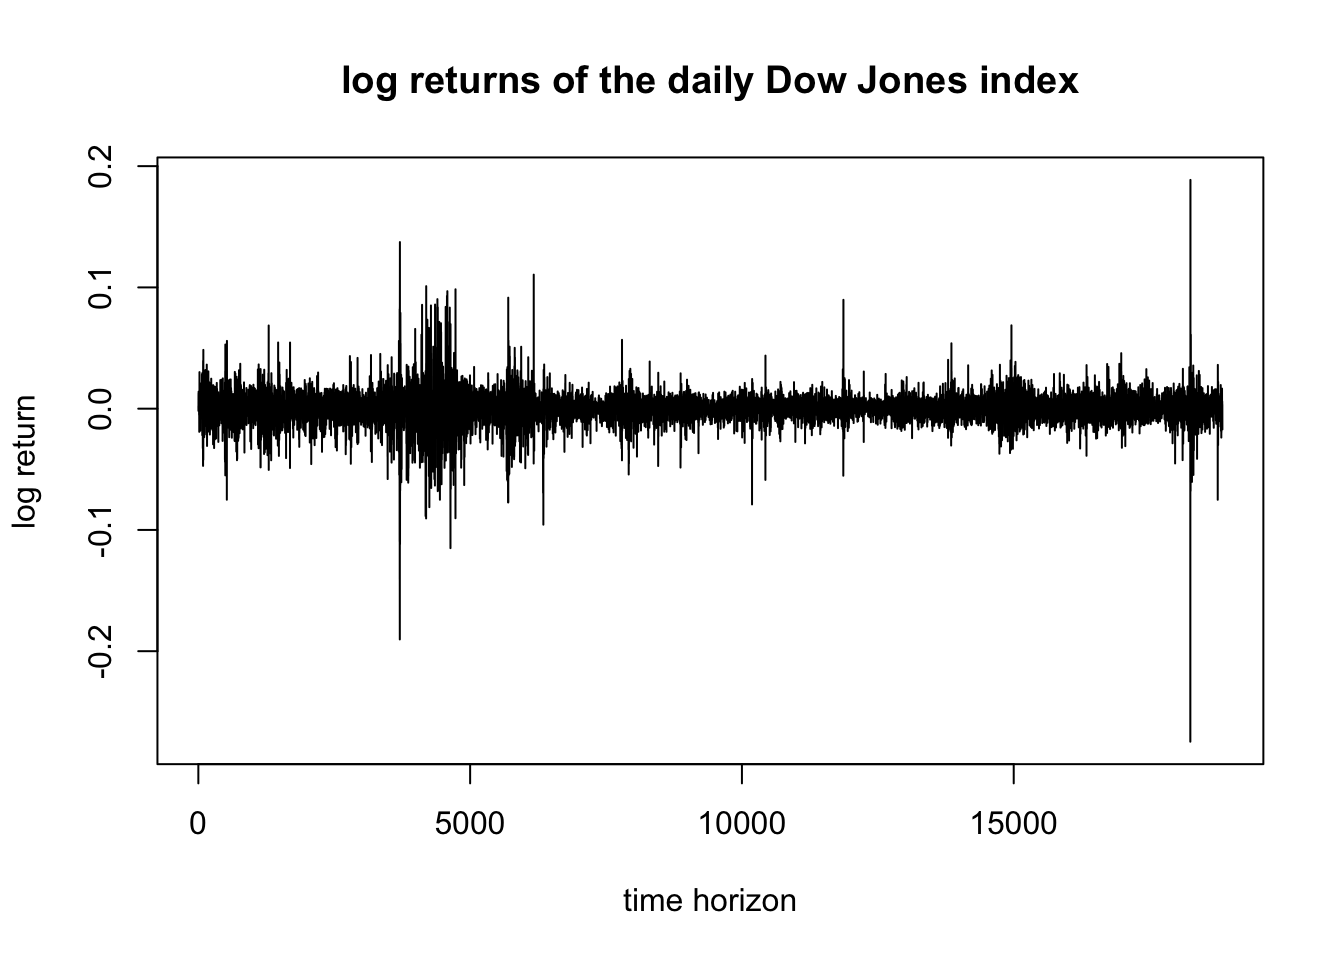
\includegraphics{PS1_RMarkdown_some_solutions_files/figure-latex/PLOT1-1.pdf}
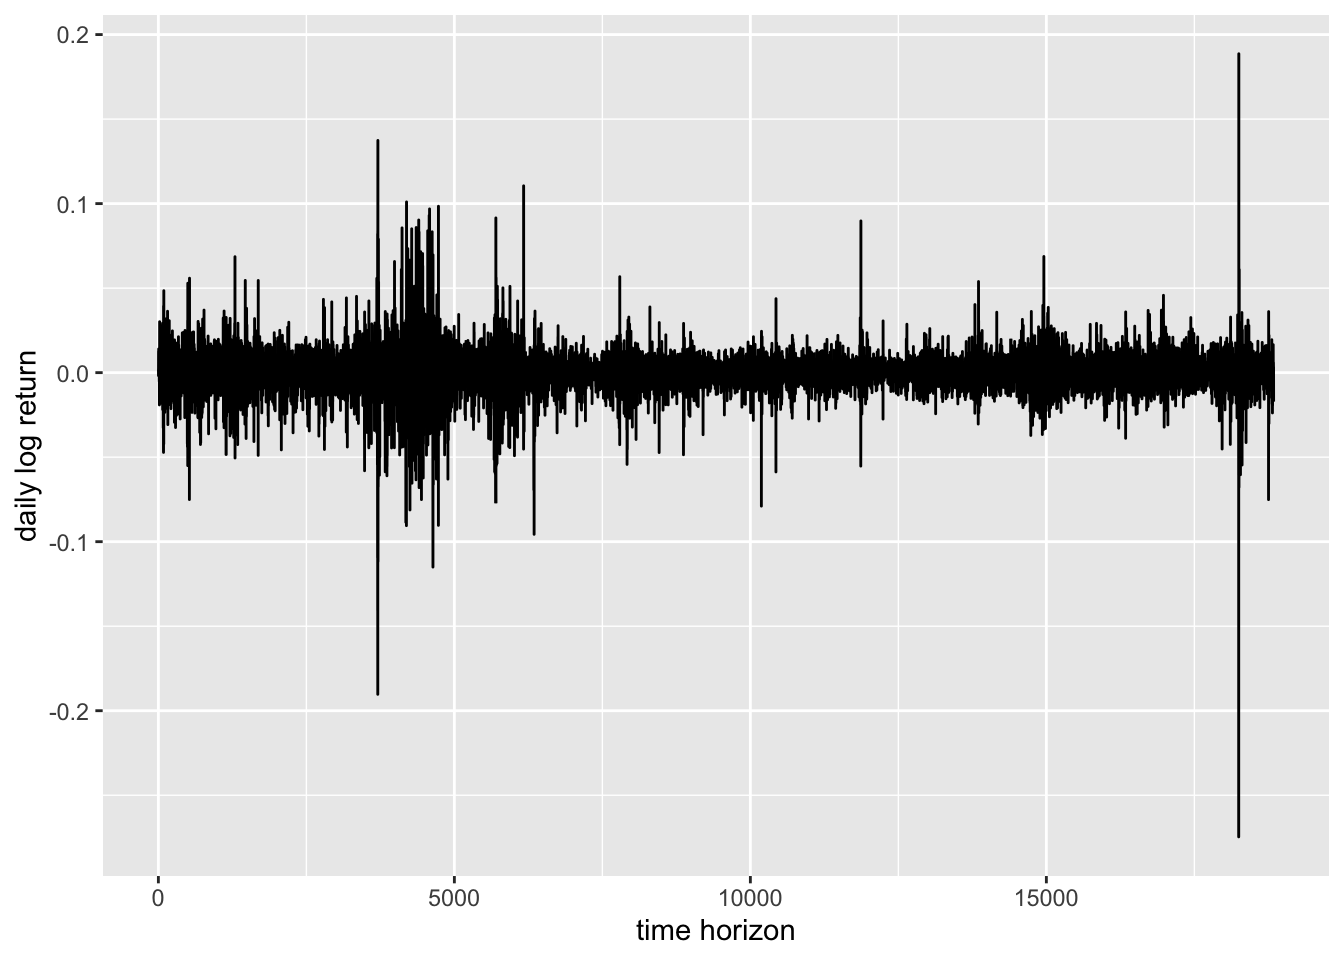
\includegraphics{PS1_RMarkdown_some_solutions_files/figure-latex/PLOT1-2.pdf}

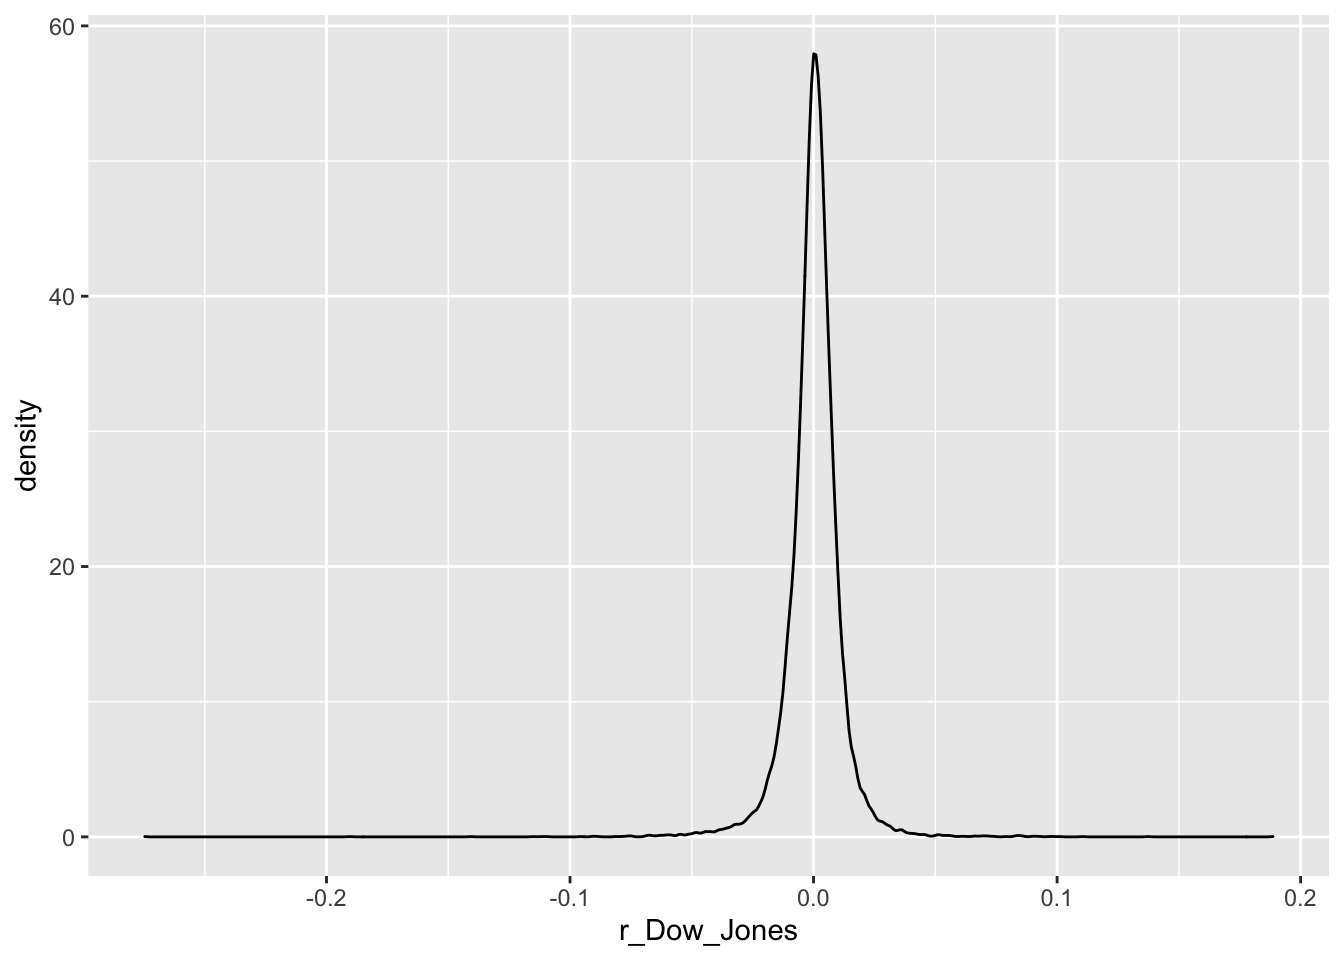
\includegraphics{PS1_RMarkdown_some_solutions_files/figure-latex/PLOT2-1.pdf}
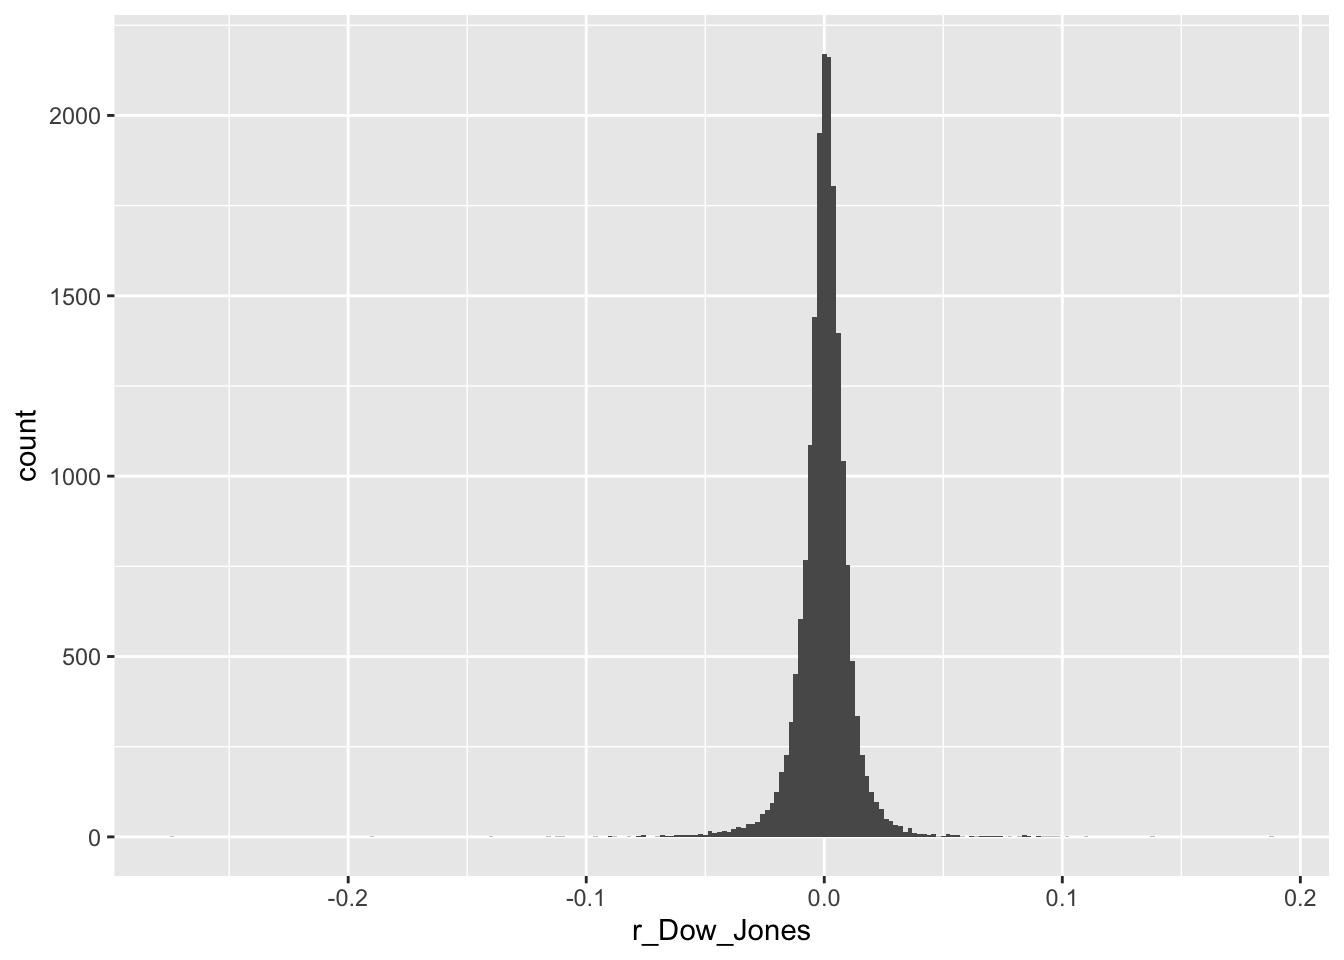
\includegraphics{PS1_RMarkdown_some_solutions_files/figure-latex/PLOT2-2.pdf}
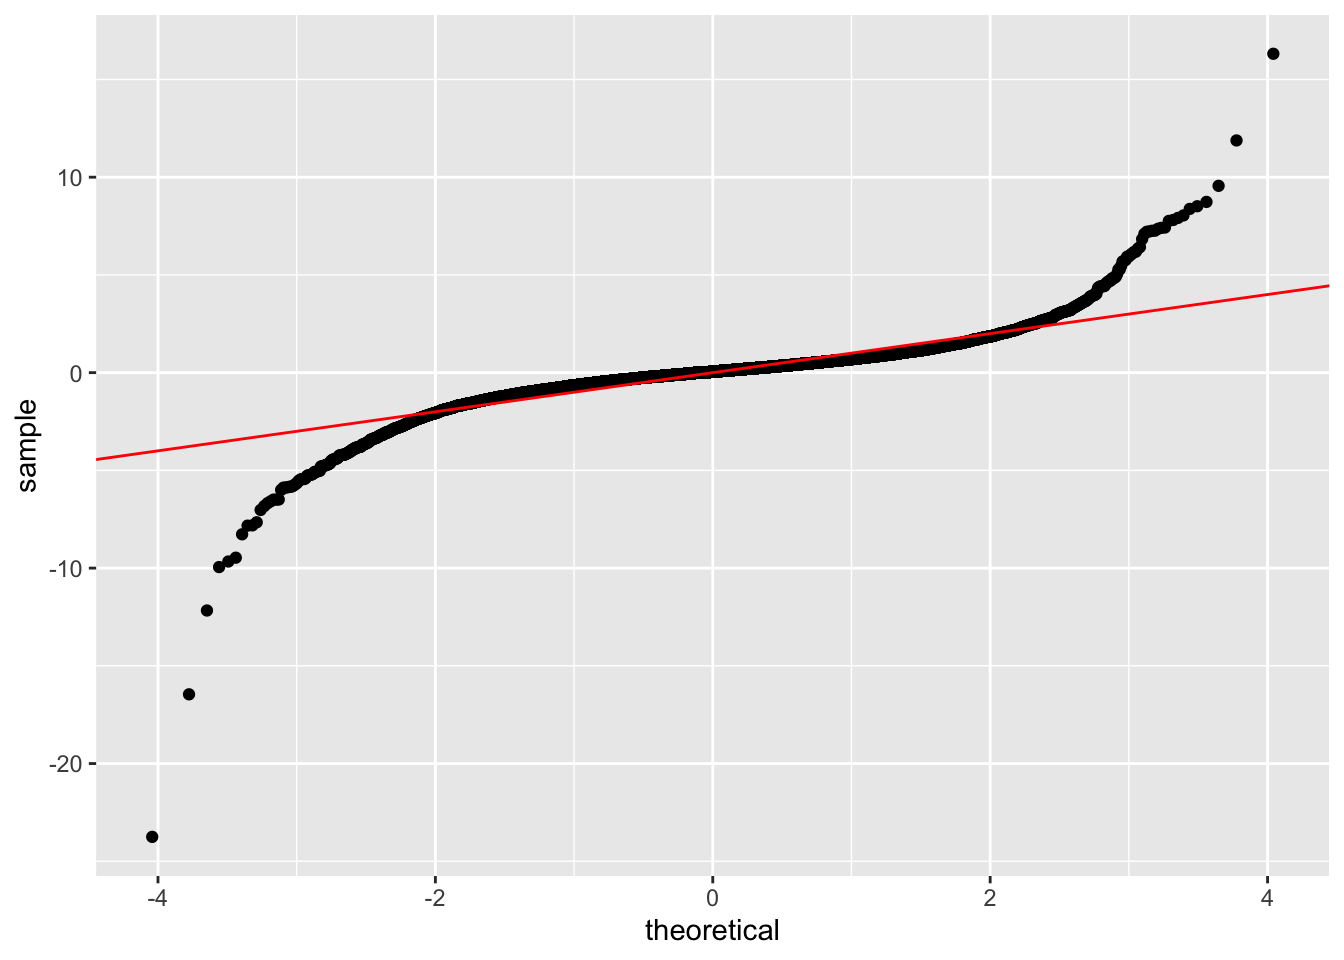
\includegraphics{PS1_RMarkdown_some_solutions_files/figure-latex/PLOT2-3.pdf}

\begin{verbatim}
## 
## Attaching package: 'psych'
\end{verbatim}

\begin{verbatim}
## The following objects are masked from 'package:ggplot2':
## 
##     %+%, alpha
\end{verbatim}

\begin{verbatim}
##    vars     n mean   sd median trimmed  mad   min  max range  skew kurtosis se
## X1    1 18839    0 0.01      0       0 0.01 -0.27 0.19  0.46 -0.96     36.6  0
\end{verbatim}

\begin{verbatim}
##    vars    n mean   sd median trimmed  mad   min  max range  skew kurtosis se
## X1    1 4686    0 0.03      0       0 0.02 -0.35 0.21  0.56 -1.09    15.06  0
\end{verbatim}

\begin{Shaded}
\begin{Highlighting}[]
\NormalTok{df }\OtherTok{=} \DecValTok{3}
\NormalTok{tmp }\OtherTok{=} \FunctionTok{ggplot}\NormalTok{(DJ\_d, }\FunctionTok{aes}\NormalTok{(}\AttributeTok{sample=}\NormalTok{r\_Dow\_Jones}\SpecialCharTok{/}\FunctionTok{sd}\NormalTok{(r\_Dow\_Jones)}\SpecialCharTok{*}\FunctionTok{sqrt}\NormalTok{(df}\SpecialCharTok{/}\NormalTok{(df}\DecValTok{{-}2}\NormalTok{))))}
\NormalTok{tmp }\SpecialCharTok{+} \FunctionTok{geom\_qq}\NormalTok{(}\AttributeTok{distribution=}\NormalTok{stats}\SpecialCharTok{::}\NormalTok{qt, }\AttributeTok{dparams=}\FunctionTok{list}\NormalTok{(}\AttributeTok{df=}\NormalTok{df)) }\SpecialCharTok{+} \FunctionTok{geom\_abline}\NormalTok{(}\FunctionTok{aes}\NormalTok{(}\AttributeTok{intercept=}\DecValTok{0}\NormalTok{,}\AttributeTok{slope=}\DecValTok{1}\NormalTok{),}\AttributeTok{color=}\StringTok{"red"}\NormalTok{)}
\end{Highlighting}
\end{Shaded}

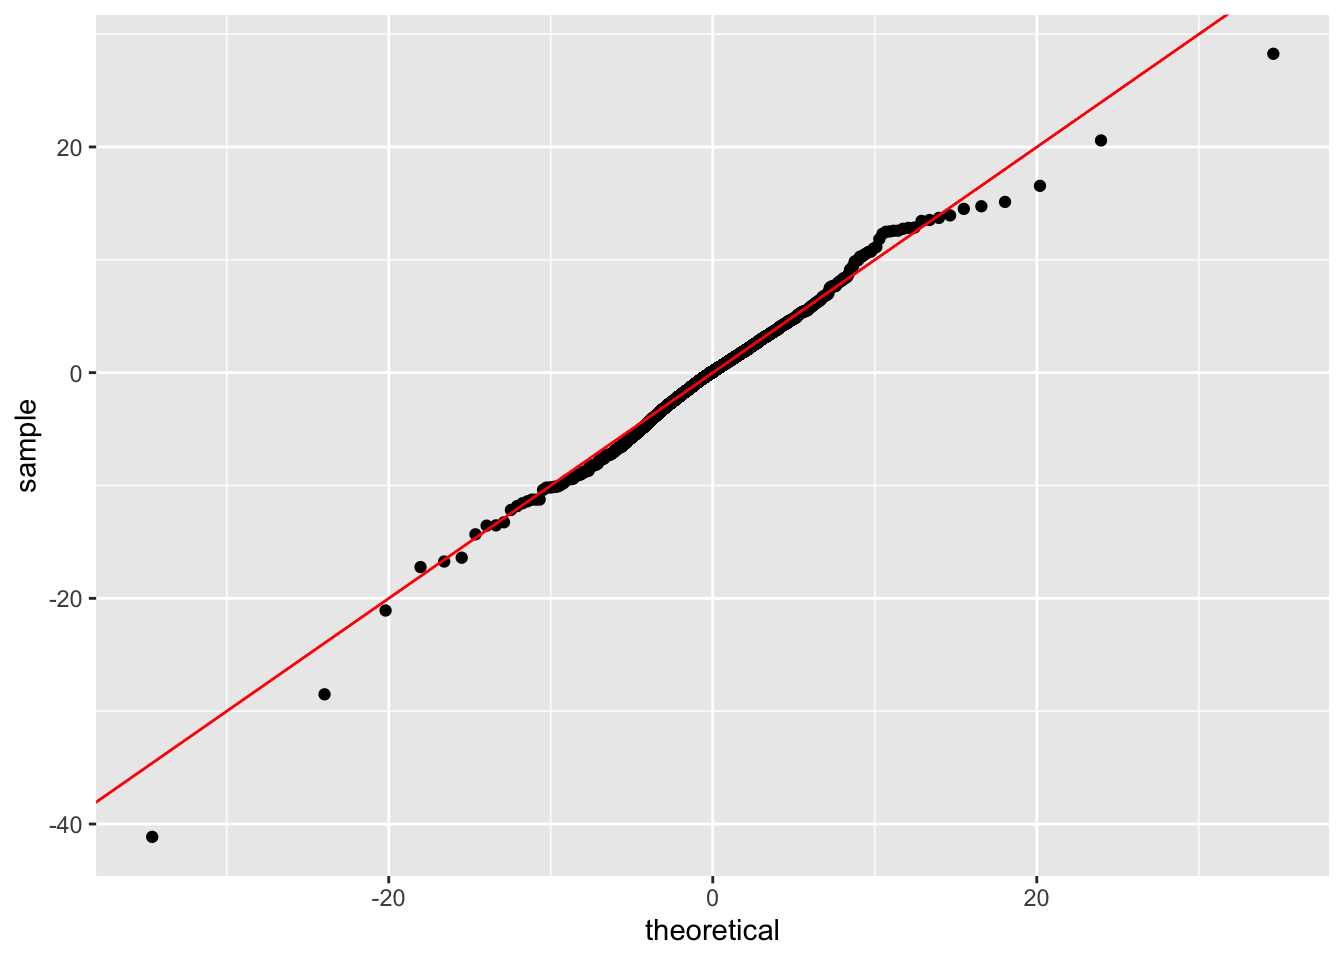
\includegraphics{PS1_RMarkdown_some_solutions_files/figure-latex/tdist-1.pdf}

\begin{Shaded}
\begin{Highlighting}[]
\CommentTok{\#qqplot(rt(length(DJ\_d$r\_Dow\_Jones),df=5),DJ\_d$r\_Dow\_Jones)}
\end{Highlighting}
\end{Shaded}

\begin{Shaded}
\begin{Highlighting}[]
\NormalTok{vq }\OtherTok{=} \FunctionTok{pnorm}\NormalTok{(vdata)}
\FunctionTok{hist}\NormalTok{(vq)}
\end{Highlighting}
\end{Shaded}

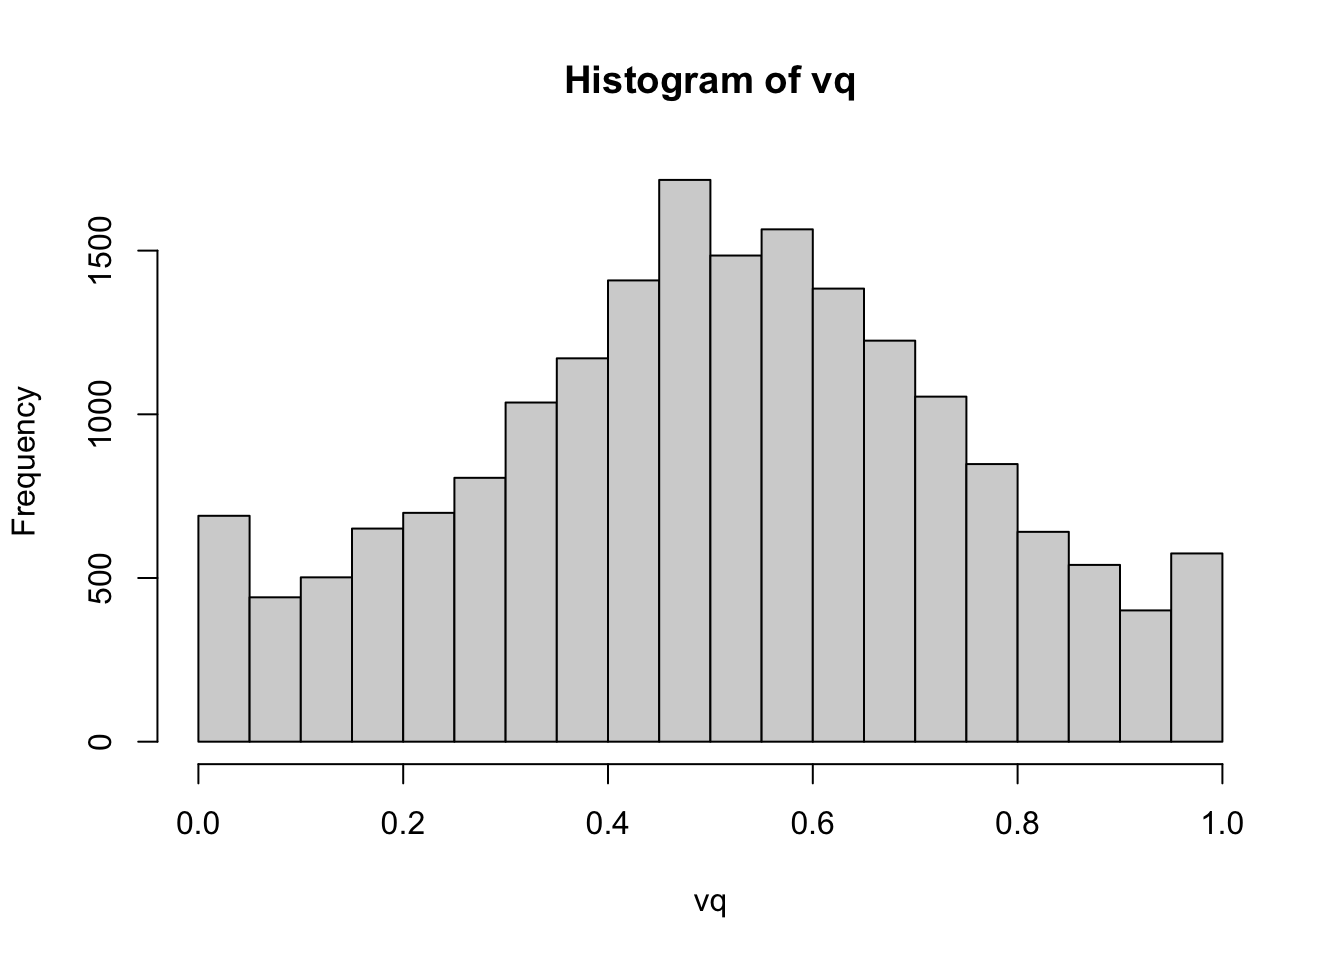
\includegraphics{PS1_RMarkdown_some_solutions_files/figure-latex/gooda-1.pdf}

\begin{Shaded}
\begin{Highlighting}[]
\FunctionTok{ggplot}\NormalTok{(}\AttributeTok{data=}\FunctionTok{tibble}\NormalTok{(vq),}\FunctionTok{aes}\NormalTok{(vq))}\SpecialCharTok{+}\FunctionTok{geom\_histogram}\NormalTok{()}
\end{Highlighting}
\end{Shaded}

\begin{verbatim}
## `stat_bin()` using `bins = 30`. Pick better value with `binwidth`.
\end{verbatim}

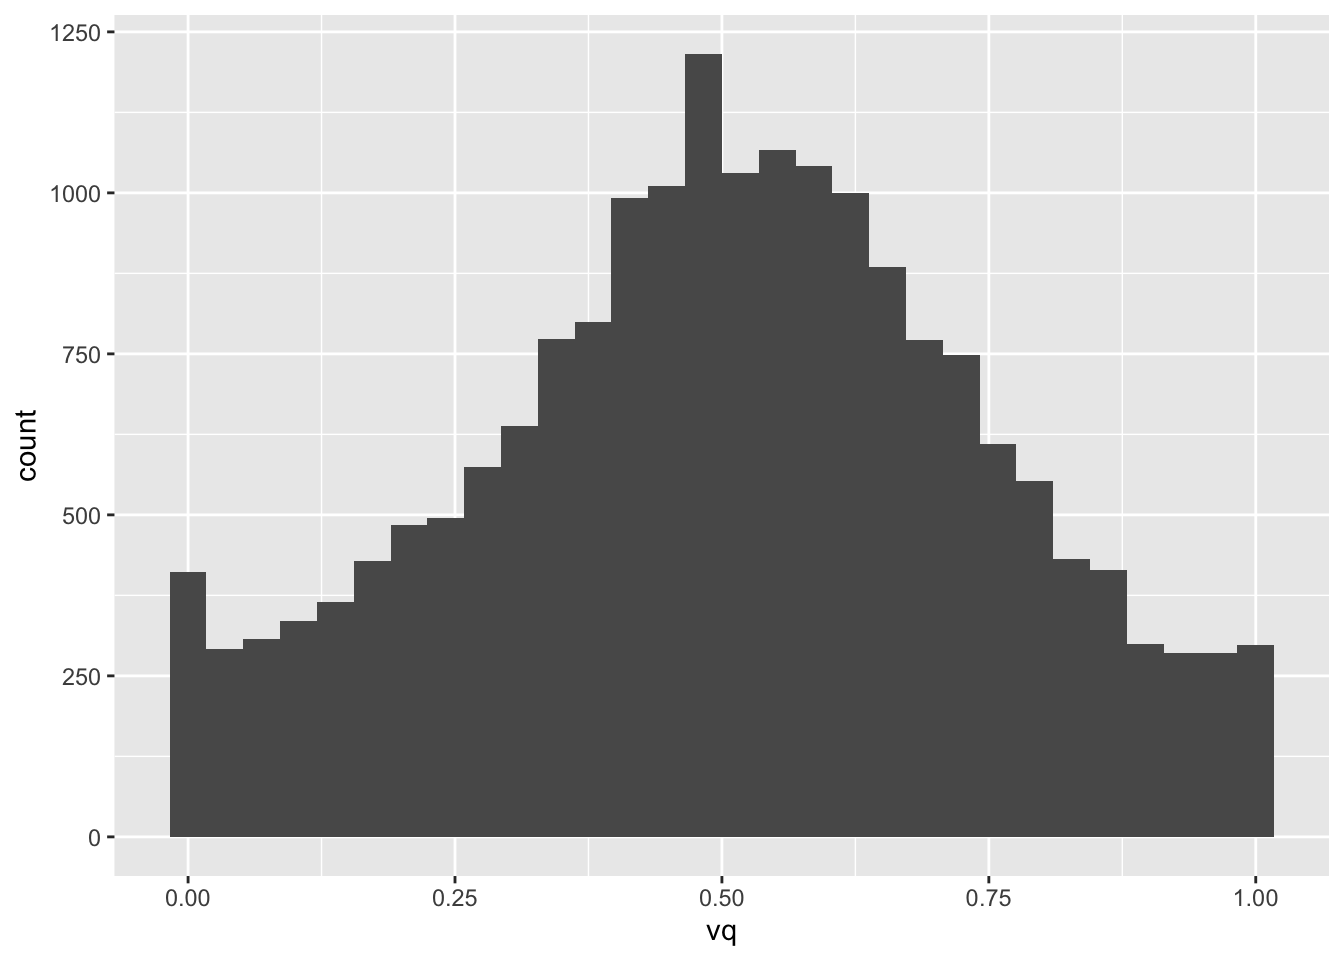
\includegraphics{PS1_RMarkdown_some_solutions_files/figure-latex/gooda-2.pdf}

\begin{Shaded}
\begin{Highlighting}[]
\NormalTok{vn }\OtherTok{=} \ConstantTok{NULL}\NormalTok{; }\ControlFlowTok{for}\NormalTok{(val }\ControlFlowTok{in}\NormalTok{ grids) vn }\OtherTok{=} \FunctionTok{c}\NormalTok{(vn,}\FunctionTok{sum}\NormalTok{(vq }\SpecialCharTok{\textless{}=}\NormalTok{ val))}
\NormalTok{vn }\OtherTok{=} \FunctionTok{c}\NormalTok{(vn[}\DecValTok{1}\NormalTok{],}\FunctionTok{diff}\NormalTok{(vn))}
\NormalTok{test }\OtherTok{=} \FunctionTok{sum}\NormalTok{((vn}\SpecialCharTok{{-}}\FunctionTok{length}\NormalTok{(vdata)}\SpecialCharTok{/}\NormalTok{ik)}\SpecialCharTok{**}\DecValTok{2}\SpecialCharTok{/}\NormalTok{(}\FunctionTok{length}\NormalTok{(vdata)}\SpecialCharTok{/}\NormalTok{ik))}
\FunctionTok{cat}\NormalTok{(}\StringTok{"test ="}\NormalTok{,test,}\StringTok{" df ="}\NormalTok{,ik}\DecValTok{{-}3}\NormalTok{,}\StringTok{" p{-}value ="}\NormalTok{,}\DecValTok{1}\SpecialCharTok{{-}}\FunctionTok{pchisq}\NormalTok{(test,}\AttributeTok{df=}\NormalTok{ik}\DecValTok{{-}3}\NormalTok{))}
\end{Highlighting}
\end{Shaded}

\begin{verbatim}
## test = 3405.87  df = 17  p-value = 0
\end{verbatim}

\begin{Shaded}
\begin{Highlighting}[]
\NormalTok{df }\OtherTok{=} \DecValTok{3}
\NormalTok{ndata }\OtherTok{=}\NormalTok{ vdata}\SpecialCharTok{*}\FunctionTok{sqrt}\NormalTok{(df}\SpecialCharTok{/}\NormalTok{(df}\DecValTok{{-}2}\NormalTok{))}
\NormalTok{vq }\OtherTok{=} \FunctionTok{pt}\NormalTok{(ndata,}\AttributeTok{df=}\DecValTok{5}\NormalTok{); }\FunctionTok{hist}\NormalTok{(vq)}
\end{Highlighting}
\end{Shaded}

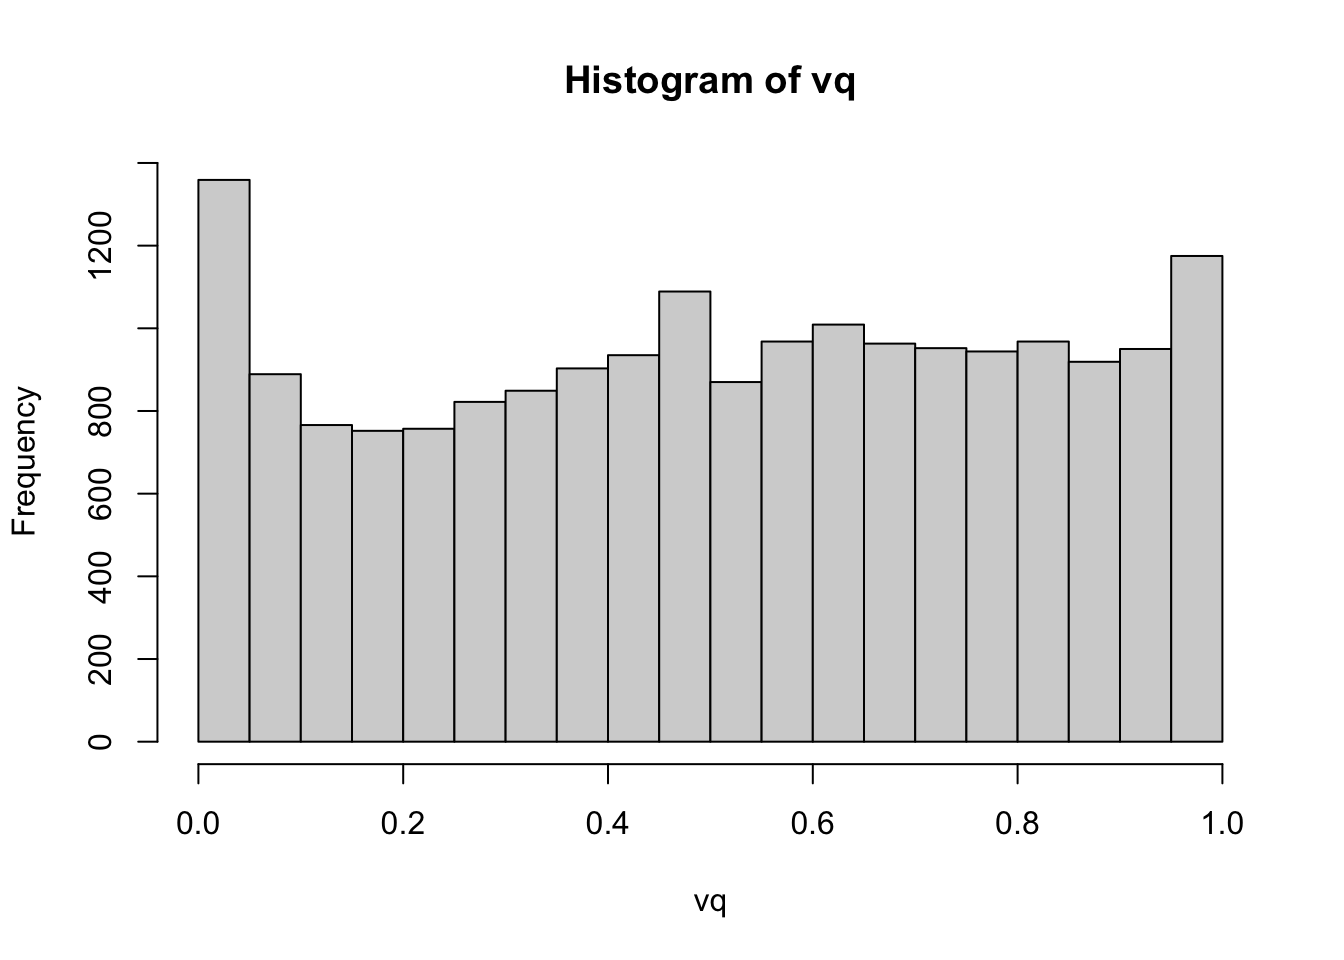
\includegraphics{PS1_RMarkdown_some_solutions_files/figure-latex/goodb-1.pdf}

\begin{Shaded}
\begin{Highlighting}[]
\NormalTok{vn }\OtherTok{=} \ConstantTok{NULL}\NormalTok{; }\ControlFlowTok{for}\NormalTok{(val }\ControlFlowTok{in}\NormalTok{ grids) vn }\OtherTok{=} \FunctionTok{c}\NormalTok{(vn,}\FunctionTok{sum}\NormalTok{(vq }\SpecialCharTok{\textless{}=}\NormalTok{ val))}
\NormalTok{vn }\OtherTok{=} \FunctionTok{c}\NormalTok{(vn[}\DecValTok{1}\NormalTok{],}\FunctionTok{diff}\NormalTok{(vn))}
\NormalTok{test }\OtherTok{=} \FunctionTok{sum}\NormalTok{((vn}\SpecialCharTok{{-}}\FunctionTok{length}\NormalTok{(vdata)}\SpecialCharTok{/}\NormalTok{ik)}\SpecialCharTok{**}\DecValTok{2}\SpecialCharTok{/}\NormalTok{(}\FunctionTok{length}\NormalTok{(vdata)}\SpecialCharTok{/}\NormalTok{ik))}
\FunctionTok{cat}\NormalTok{(}\StringTok{"test ="}\NormalTok{,test,}\StringTok{" df ="}\NormalTok{,ik}\DecValTok{{-}3}\NormalTok{,}\StringTok{" p{-}value ="}\NormalTok{,}\DecValTok{1}\SpecialCharTok{{-}}\FunctionTok{pchisq}\NormalTok{(test,}\AttributeTok{df=}\NormalTok{ik}\DecValTok{{-}3}\NormalTok{))}
\end{Highlighting}
\end{Shaded}

\begin{verbatim}
## test = 414.7555  df = 17  p-value = 0
\end{verbatim}

\begin{Shaded}
\begin{Highlighting}[]
\NormalTok{alpha }\OtherTok{=} \FloatTok{0.1514736}
\NormalTok{sigma }\OtherTok{=} \FloatTok{4.0013995}
\NormalTok{ndata }\OtherTok{=}\NormalTok{ vdata }\SpecialCharTok{*} \FunctionTok{sqrt}\NormalTok{((}\DecValTok{1}\SpecialCharTok{{-}}\NormalTok{alpha) }\SpecialCharTok{+}\NormalTok{ alpha}\SpecialCharTok{*}\NormalTok{sigma}\SpecialCharTok{**}\DecValTok{2}\NormalTok{)}
\NormalTok{vq }\OtherTok{=}\NormalTok{ (}\DecValTok{1}\SpecialCharTok{{-}}\NormalTok{alpha)}\SpecialCharTok{*}\FunctionTok{pnorm}\NormalTok{(ndata) }\SpecialCharTok{+}\NormalTok{ alpha}\SpecialCharTok{*}\FunctionTok{pnorm}\NormalTok{(ndata,}\AttributeTok{sd=}\NormalTok{sigma); }\FunctionTok{hist}\NormalTok{(vq)}
\end{Highlighting}
\end{Shaded}

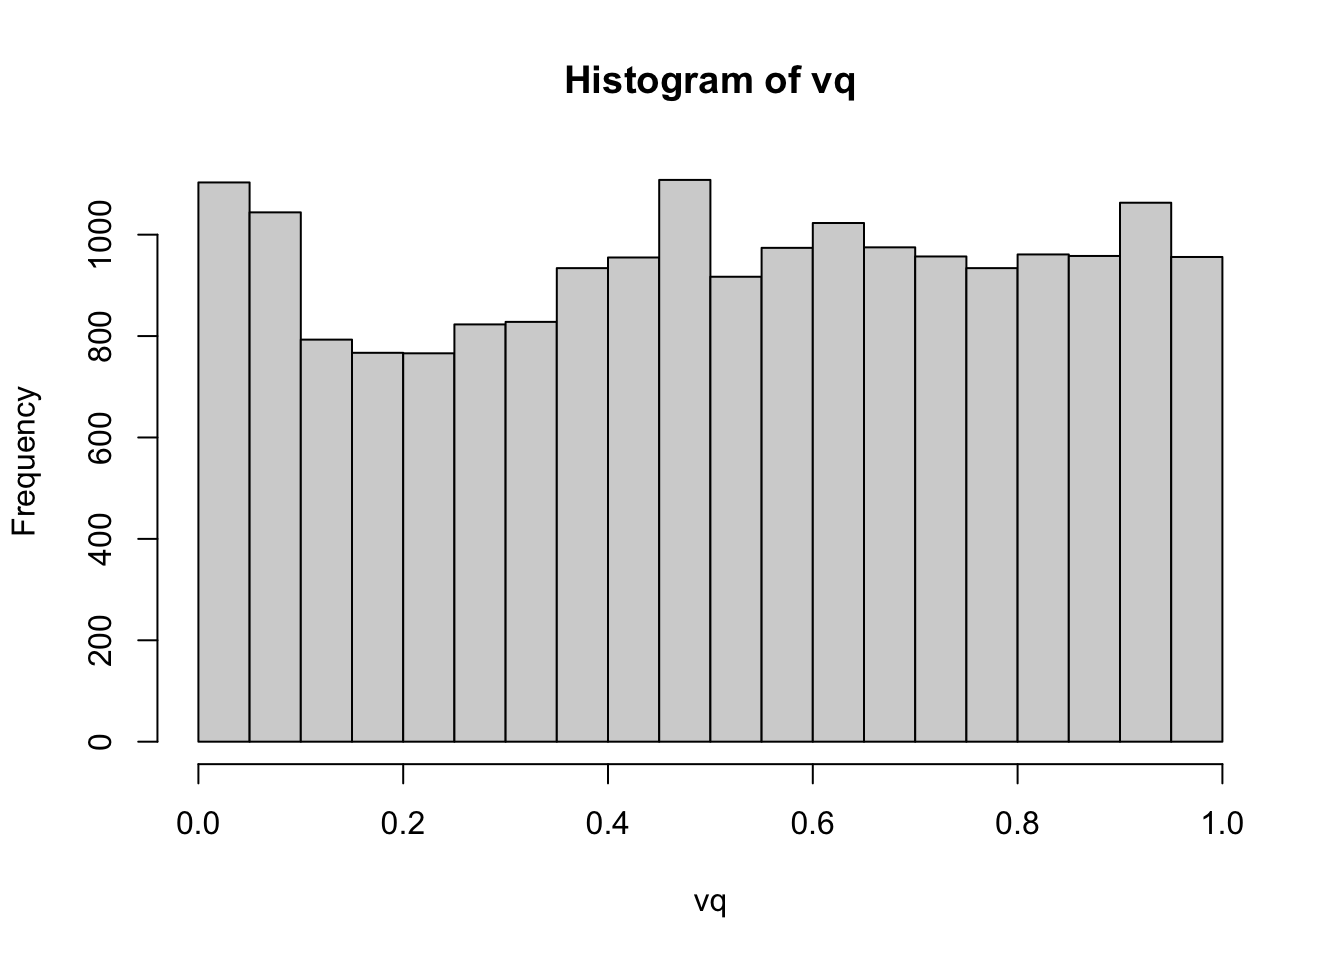
\includegraphics{PS1_RMarkdown_some_solutions_files/figure-latex/unnamed-chunk-1-1.pdf}

\begin{Shaded}
\begin{Highlighting}[]
\NormalTok{vn }\OtherTok{=} \ConstantTok{NULL}\NormalTok{; }\ControlFlowTok{for}\NormalTok{(val }\ControlFlowTok{in}\NormalTok{ grids) vn }\OtherTok{=} \FunctionTok{c}\NormalTok{(vn,}\FunctionTok{sum}\NormalTok{(vq }\SpecialCharTok{\textless{}=}\NormalTok{ val))}
\NormalTok{vn }\OtherTok{=} \FunctionTok{c}\NormalTok{(vn[}\DecValTok{1}\NormalTok{],}\FunctionTok{diff}\NormalTok{(vn))}
\NormalTok{test }\OtherTok{=} \FunctionTok{sum}\NormalTok{((vn}\SpecialCharTok{{-}}\FunctionTok{length}\NormalTok{(vdata)}\SpecialCharTok{/}\NormalTok{ik)}\SpecialCharTok{**}\DecValTok{2}\SpecialCharTok{/}\NormalTok{(}\FunctionTok{length}\NormalTok{(vdata)}\SpecialCharTok{/}\NormalTok{ik))}
\FunctionTok{cat}\NormalTok{(}\StringTok{"test ="}\NormalTok{,test,}\StringTok{" df ="}\NormalTok{,ik}\DecValTok{{-}3}\NormalTok{,}\StringTok{" p{-}value ="}\NormalTok{,}\DecValTok{1}\SpecialCharTok{{-}}\FunctionTok{pchisq}\NormalTok{(test,}\AttributeTok{df=}\NormalTok{ik}\DecValTok{{-}3}\NormalTok{))}
\end{Highlighting}
\end{Shaded}

\begin{verbatim}
## test = 212.4475  df = 17  p-value = 0
\end{verbatim}

Write a function for minimization to choose the optimal pair for
\(\alpha\) and \(\sigma\).

\begin{Shaded}
\begin{Highlighting}[]
\NormalTok{func }\OtherTok{\textless{}{-}} \ControlFlowTok{function}\NormalTok{(vx)\{}
\NormalTok{  alpha }\OtherTok{=}\NormalTok{ vx[}\DecValTok{1}\NormalTok{]}
\NormalTok{  sigma }\OtherTok{=}\NormalTok{ vx[}\DecValTok{2}\NormalTok{]}
\NormalTok{  ndata }\OtherTok{=}\NormalTok{ vdata}\SpecialCharTok{*}\FunctionTok{sqrt}\NormalTok{((}\DecValTok{1}\SpecialCharTok{{-}}\NormalTok{alpha) }\SpecialCharTok{+}\NormalTok{ alpha}\SpecialCharTok{*}\NormalTok{sigma}\SpecialCharTok{**}\DecValTok{2}\NormalTok{)}

\NormalTok{  vq }\OtherTok{=}\NormalTok{ (}\DecValTok{1}\SpecialCharTok{{-}}\NormalTok{alpha)}\SpecialCharTok{*}\FunctionTok{pnorm}\NormalTok{(ndata) }\SpecialCharTok{+}\NormalTok{ alpha}\SpecialCharTok{*}\FunctionTok{pnorm}\NormalTok{(ndata,}\AttributeTok{sd=}\NormalTok{sigma)}
\NormalTok{  vn }\OtherTok{=} \ConstantTok{NULL}\NormalTok{; }\ControlFlowTok{for}\NormalTok{(val }\ControlFlowTok{in}\NormalTok{ grids) vn }\OtherTok{=} \FunctionTok{c}\NormalTok{(vn,}\FunctionTok{sum}\NormalTok{(vq }\SpecialCharTok{\textless{}=}\NormalTok{ val))}
\NormalTok{  vn }\OtherTok{=} \FunctionTok{c}\NormalTok{(vn[}\DecValTok{1}\NormalTok{],}\FunctionTok{diff}\NormalTok{(vn))}
  \FunctionTok{return}\NormalTok{(}\FunctionTok{sum}\NormalTok{((vn}\SpecialCharTok{{-}}\FunctionTok{length}\NormalTok{(vdata)}\SpecialCharTok{/}\NormalTok{ik)}\SpecialCharTok{**}\DecValTok{2}\SpecialCharTok{/}\NormalTok{(}\FunctionTok{length}\NormalTok{(vdata)}\SpecialCharTok{/}\NormalTok{ik)))}
\NormalTok{\}}

\FunctionTok{func}\NormalTok{(}\FunctionTok{c}\NormalTok{(}\FloatTok{0.15}\NormalTok{,}\DecValTok{4}\NormalTok{))}
\end{Highlighting}
\end{Shaded}

\begin{verbatim}
## [1] 212.7936
\end{verbatim}

\begin{Shaded}
\begin{Highlighting}[]
\FunctionTok{optim}\NormalTok{(}\AttributeTok{par=}\FunctionTok{c}\NormalTok{(}\FloatTok{0.15}\NormalTok{,}\DecValTok{4}\NormalTok{),}\AttributeTok{fn=}\NormalTok{func,}\AttributeTok{method=}\StringTok{"BFGS"}\NormalTok{)}
\end{Highlighting}
\end{Shaded}

\begin{verbatim}
## Warning in sqrt((1 - alpha) + alpha * sigma^2): NaNs produced

## Warning in sqrt((1 - alpha) + alpha * sigma^2): NaNs produced

## Warning in sqrt((1 - alpha) + alpha * sigma^2): NaNs produced

## Warning in sqrt((1 - alpha) + alpha * sigma^2): NaNs produced

## Warning in sqrt((1 - alpha) + alpha * sigma^2): NaNs produced

## Warning in sqrt((1 - alpha) + alpha * sigma^2): NaNs produced

## Warning in sqrt((1 - alpha) + alpha * sigma^2): NaNs produced

## Warning in sqrt((1 - alpha) + alpha * sigma^2): NaNs produced
\end{verbatim}

\begin{verbatim}
## $par
## [1] 0.1515383 4.0008180
## 
## $value
## [1] 212.4475
## 
## $counts
## function gradient 
##       54        2 
## 
## $convergence
## [1] 0
## 
## $message
## NULL
\end{verbatim}

\begin{Shaded}
\begin{Highlighting}[]
\FunctionTok{optim}\NormalTok{(}\AttributeTok{par=}\FunctionTok{c}\NormalTok{(}\FloatTok{0.15}\NormalTok{,}\DecValTok{4}\NormalTok{),}\AttributeTok{fn=}\NormalTok{func,}\AttributeTok{method=}\StringTok{"L{-}BFGS{-}B"}\NormalTok{,}\AttributeTok{lower=}\FunctionTok{c}\NormalTok{(}\DecValTok{0}\NormalTok{,}\DecValTok{0}\NormalTok{),}\AttributeTok{upper=}\FunctionTok{c}\NormalTok{(}\DecValTok{1}\NormalTok{,}\DecValTok{10}\NormalTok{)) }
\end{Highlighting}
\end{Shaded}

\begin{verbatim}
## $par
## [1] 0.1752619 3.7378776
## 
## $value
## [1] 190.9963
## 
## $counts
## function gradient 
##      148      148 
## 
## $convergence
## [1] 52
## 
## $message
## [1] "ERROR: ABNORMAL_TERMINATION_IN_LNSRCH"
\end{verbatim}

\begin{Shaded}
\begin{Highlighting}[]
\NormalTok{atmp }\OtherTok{=} \FunctionTok{seq}\NormalTok{(}\AttributeTok{from=}\FloatTok{0.05}\NormalTok{, }\AttributeTok{to=}\NormalTok{.}\DecValTok{95}\NormalTok{, }\AttributeTok{length.out=}\DecValTok{40}\NormalTok{)}
\NormalTok{stmp }\OtherTok{=} \FunctionTok{seq}\NormalTok{(}\AttributeTok{from=}\DecValTok{1}\NormalTok{, }\AttributeTok{to=}\DecValTok{10}\NormalTok{, }\AttributeTok{length.out=}\DecValTok{50}\NormalTok{)}
\NormalTok{tmp }\OtherTok{=} \FunctionTok{expand.grid}\NormalTok{(atmp,stmp)}
\NormalTok{res }\OtherTok{=} \FunctionTok{apply}\NormalTok{(tmp,}\DecValTok{1}\NormalTok{,func)}
\NormalTok{res }\OtherTok{=} \FunctionTok{t}\NormalTok{(}\FunctionTok{matrix}\NormalTok{(res, }\AttributeTok{nrow=}\FunctionTok{length}\NormalTok{(atmp)))}

\FunctionTok{library}\NormalTok{(plotly)}
\end{Highlighting}
\end{Shaded}

\begin{verbatim}
## 
## Attaching package: 'plotly'
\end{verbatim}

\begin{verbatim}
## The following object is masked from 'package:ggplot2':
## 
##     last_plot
\end{verbatim}

\begin{verbatim}
## The following object is masked from 'package:stats':
## 
##     filter
\end{verbatim}

\begin{verbatim}
## The following object is masked from 'package:graphics':
## 
##     layout
\end{verbatim}

\begin{Shaded}
\begin{Highlighting}[]
\NormalTok{ret }\OtherTok{=} \FunctionTok{plot\_ly}\NormalTok{(}\AttributeTok{x=}\NormalTok{atmp, }\AttributeTok{y=}\NormalTok{stmp, }\AttributeTok{z=}\NormalTok{res) }\SpecialCharTok{\%\textgreater{}\%} \FunctionTok{add\_surface}\NormalTok{() }\SpecialCharTok{\%\textgreater{}\%}
  \FunctionTok{layout}\NormalTok{(}\AttributeTok{scene=}\FunctionTok{list}\NormalTok{(}\AttributeTok{xaxis=}\FunctionTok{list}\NormalTok{(}\AttributeTok{title=}\StringTok{\textquotesingle{}alpha\textquotesingle{}}\NormalTok{), }\AttributeTok{yaxis=}\FunctionTok{list}\NormalTok{(}\AttributeTok{title=}\StringTok{\textquotesingle{}sigma\textquotesingle{}}\NormalTok{), }\AttributeTok{zaxis=}\FunctionTok{list}\NormalTok{(}\AttributeTok{title=}\StringTok{\textquotesingle{}function\textquotesingle{}}\NormalTok{)))}
\NormalTok{ret}
\end{Highlighting}
\end{Shaded}

\includegraphics{PS1_RMarkdown_some_solutions_files/figure-latex/unnamed-chunk-4-1.pdf}

\hypertarget{dynamical-properties-of-financial-return-series}{%
\subsection{Dynamical properties of financial return
series}\label{dynamical-properties-of-financial-return-series}}

\begin{Shaded}
\begin{Highlighting}[]
\NormalTok{lret }\OtherTok{=} \FunctionTok{apply}\NormalTok{(}\FunctionTok{log}\NormalTok{(data),}\DecValTok{2}\NormalTok{,diff)}
\FunctionTok{summary}\NormalTok{(lret)}
\end{Highlighting}
\end{Shaded}

\begin{verbatim}
##     DAXINDX              FRCAC40           FTSE100          
##  Min.   :-0.1370990   Min.   :-0.1014   Min.   :-0.1302860  
##  1st Qu.:-0.0053976   1st Qu.:-0.0060   1st Qu.:-0.0045157  
##  Median : 0.0002581   Median : 0.0000   Median : 0.0002738  
##  Mean   : 0.0003493   Mean   : 0.0003   Mean   : 0.0004102  
##  3rd Qu.: 0.0070188   3rd Qu.: 0.0069   3rd Qu.: 0.0058174  
##  Max.   : 0.0728754   Max.   : 0.0823   Max.   : 0.0759697  
##                       NA's   :393                           
##     HNGKNGI               NIKKEI              SNGALLS          
##  Min.   :-0.4054220   Min.   :-1.614e-01   Min.   :-0.0940305  
##  1st Qu.:-0.0053347   1st Qu.:-6.014e-03   1st Qu.:-0.0041041  
##  Median : 0.0002220   Median : 0.000e+00   Median : 0.0000000  
##  Mean   : 0.0005713   Mean   : 4.991e-05   Mean   : 0.0001921  
##  3rd Qu.: 0.0079703   3rd Qu.: 6.380e-03   3rd Qu.: 0.0047405  
##  Max.   : 0.1724710   Max.   : 1.243e-01   Max.   : 0.1431300  
##                                                                
##      SPCOMP          
##  Min.   :-0.2283303  
##  1st Qu.:-0.0033884  
##  Median : 0.0003843  
##  Mean   : 0.0004885  
##  3rd Qu.: 0.0049146  
##  Max.   : 0.0870888  
## 
\end{verbatim}

\begin{Shaded}
\begin{Highlighting}[]
\FunctionTok{matplot}\NormalTok{(lret,}\AttributeTok{type=}\StringTok{\textquotesingle{}l\textquotesingle{}}\NormalTok{,}\AttributeTok{ylab=}\StringTok{\textquotesingle{}log returns\textquotesingle{}}\NormalTok{,}\AttributeTok{xlab=}\StringTok{\textquotesingle{}time horizon\textquotesingle{}}\NormalTok{)}
\end{Highlighting}
\end{Shaded}

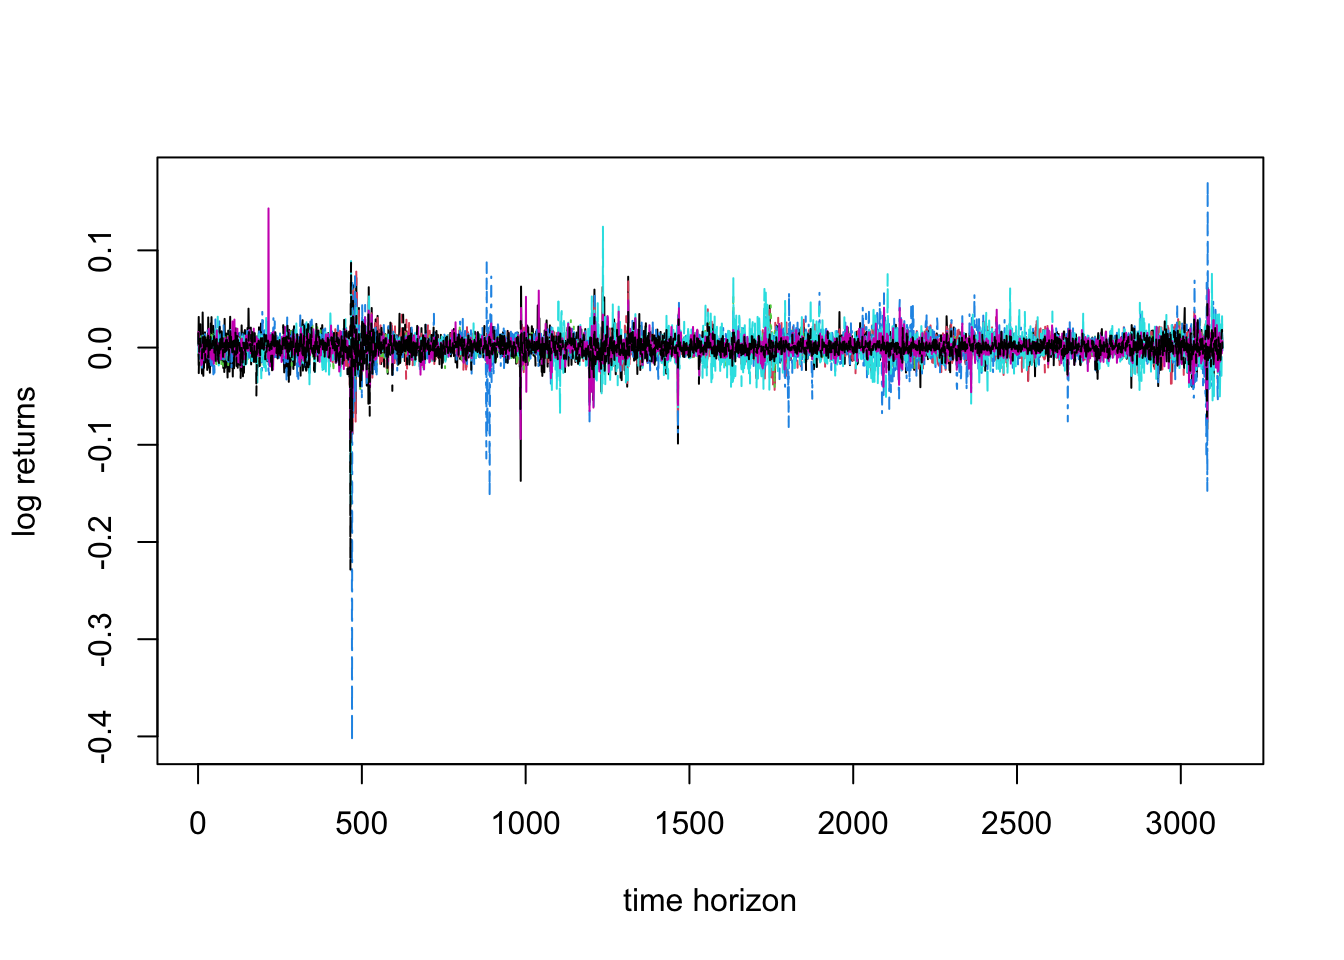
\includegraphics{PS1_RMarkdown_some_solutions_files/figure-latex/unnamed-chunk-5-1.pdf}

\begin{Shaded}
\begin{Highlighting}[]
\FunctionTok{sum}\NormalTok{(}\FunctionTok{is.na}\NormalTok{(lret[,}\StringTok{\textquotesingle{}FRCAC40\textquotesingle{}}\NormalTok{]))}
\end{Highlighting}
\end{Shaded}

\begin{verbatim}
## [1] 393
\end{verbatim}

\begin{Shaded}
\begin{Highlighting}[]
\NormalTok{LB }\OtherTok{\textless{}{-}} \ControlFlowTok{function}\NormalTok{(vx,lag,ip)\{}
\NormalTok{  tmp }\OtherTok{=} \FunctionTok{acf}\NormalTok{(vx,}\AttributeTok{lag.max=}\NormalTok{lag,}\AttributeTok{plot=}\NormalTok{F)}\SpecialCharTok{$}\NormalTok{acf}
\NormalTok{  tmp }\OtherTok{=}\NormalTok{ tmp[}\DecValTok{2}\SpecialCharTok{:}\NormalTok{(lag}\SpecialCharTok{+}\DecValTok{1}\NormalTok{)]}\SpecialCharTok{**}\DecValTok{2}
\NormalTok{  test }\OtherTok{=} \FunctionTok{sum}\NormalTok{(tmp}\SpecialCharTok{/}\NormalTok{(}\FunctionTok{length}\NormalTok{(vx)}\SpecialCharTok{{-}}\DecValTok{1}\SpecialCharTok{:}\NormalTok{lag))}\SpecialCharTok{*}\FunctionTok{length}\NormalTok{(vx)}\SpecialCharTok{*}\NormalTok{(}\FunctionTok{length}\NormalTok{(vx)}\SpecialCharTok{+}\DecValTok{2}\NormalTok{)}
  \FunctionTok{return}\NormalTok{(}\FunctionTok{list}\NormalTok{(}\AttributeTok{test=}\NormalTok{test, }\AttributeTok{pval=}\DecValTok{1}\SpecialCharTok{{-}}\FunctionTok{pchisq}\NormalTok{(test,}\AttributeTok{df=}\NormalTok{lag}\SpecialCharTok{{-}}\NormalTok{ip)))}
\NormalTok{\}}

\NormalTok{tmp }\OtherTok{=} \DecValTok{6}
\FunctionTok{LB}\NormalTok{(}\AttributeTok{vx=}\NormalTok{lret[}\SpecialCharTok{!}\FunctionTok{is.na}\NormalTok{(lret[,tmp]),tmp],}\AttributeTok{lag=}\DecValTok{100}\NormalTok{,}\AttributeTok{ip=}\DecValTok{0}\NormalTok{)}
\end{Highlighting}
\end{Shaded}

\begin{verbatim}
## $test
## [1] 202.3019
## 
## $pval
## [1] 6.465107e-09
\end{verbatim}

\end{document}
